%==============================================================================
% Sjabloon onderzoeksvoorstel bachelorproef
%==============================================================================
% Gebaseerd op LaTeX-sjabloon ‘Stylish Article’ (zie voorstel.cls)
% Auteur: Jens Buysse, Bert Van Vreckem
%
% Compileren in TeXstudio:
%
% - Zorg dat Biber de bibliografie compileert (en niet Biblatex)
%   Options > Configure > Build > Default Bibliography Tool: "txs:///biber"
% - F5 om te compileren en het resultaat te bekijken.
% - Als de bibliografie niet zichtbaar is, probeer dan F5 - F8 - F5
%   Met F8 compileer je de bibliografie apart.
%
% Als je JabRef gebruikt voor het bijhouden van de bibliografie, zorg dan
% dat je in ``biblatex''-modus opslaat: File > Switch to BibLaTeX mode.

\documentclass{voorstel}

\usepackage{lipsum}
\usepackage{cfr-lm}
\usepackage{graphicx}
\graphicspath{ {./} }
%------------------------------------------------------------------------------
% Metadata over het voorstel
%------------------------------------------------------------------------------

%---------- Titel & auteur ----------------------------------------------------

% TODO: geef werktitel van je eigen voorstel op
\PaperTitle{How the change detection strategy affects performance in Angular applications with high-frequency updates}
\PaperType{Research proposal bachelor's thesis 2020-2021} % Type document

% TODO: vul je eigen naam in als auteur, geef ook je emailadres mee!
\Authors{Duchatelet Thomas\textsuperscript{1}} % Authors
\CoPromotor{Bonnie Brennan\textsuperscript{2} (Angular Nation)}
\affiliation{\textbf{Contact:}
  \textsuperscript{1} \href{mailto:thomas.duchatelet.y3284@student.hogent.be}{thomas.duchatelet.y3284@student.hogent.be};
  \textsuperscript{2} \href{mailto:bjbrennan75@gmail.com}{bjbrennan75@gmail.com};
}

%---------- Abstract ----------------------------------------------------------
\renewcommand{\abstractname}{Abstract} % Defines the abstracts heading name
\Abstract{
Angular is a widely used web-framework and is a popular choice for developing all kinds of webapplications. Since Angular can be used to build reactive platforms, it might be suitable for realtime monitoring dashboards. Since humanity constantly tries to improve their tools, modern technologies are implemented for providing insights on big amounts of data. With the rise of the 'Internet of Things', the demand for realtime monitoring dashboards is also increasing. As IoT devices most of the time change state frequently, the default change detection strategy might not be the best solution for this case. Each strategy will be implemented and tested with high-frequency updates to investigate the effect of alternative strategies on the performance of the application. After comparing each scenario, it is expected to illustrate that performance can be maximized by implementing an alternative change detection strategy. This could lead to more responsive webapplications and more visually pleasing dashboards.

This thesis will be mentored by Bonnie Brennan (Angular Nation) and will therefore be written in English.
}


%---------- Onderzoeksdomein en sleutelwoorden --------------------------------
% TODO: Sleutelwoorden:
%
% Het eerste sleutelwoord beschrijft het onderzoeksdomein. Je kan kiezen uit
% deze lijst:
%
% - Mobiele applicatieontwikkeling
% - Webapplicatieontwikkeling
% - Applicatieontwikkeling (andere)
% - Systeembeheer
% - Netwerkbeheer
% - Mainframe
% - E-business
% - Databanken en big data
% - Machineleertechnieken en kunstmatige intelligentie
% - Andere (specifieer)
%
% De andere sleutelwoorden zijn vrij te kiezen

\Keywords{Web application development. Angular --- Change detection --- Performance} % Keywords
\newcommand{\keywordname}{Keywords} % Defines the keywords heading name

%---------- Titel, inhoud -----------------------------------------------------

\begin{document}
\renewcommand{\abstractname}{Abstract} % Defines the abstracts heading name
\renewcommand{\contentsname}{Table of contents} % Defines the abstracts heading name
\renewcommand\refname{References}
\flushbottom % Makes all text pages the same height
\maketitle % Print the title and abstract box
\tableofcontents % Print the contents section
\thispagestyle{empty} % Removes page numbering from the first page

%------------------------------------------------------------------------------
% Hoofdtekst
%------------------------------------------------------------------------------

% De hoofdtekst van het voorstel zit in een apart bestand, zodat het makkelijk
% kan opgenomen worden in de bijlagen van de bachelorproef zelf.
%---------- Inleiding ---------------------------------------------------------

\section{Introduction} % The \section*{} command stops section numbering
\label{sec:introductie}

Thanks to the 'Internet of Things' (IoT),all sorts of devices can nowadays be connected to measure a wide range of events and collect loads of data using sensors. This data can be visualized on dashboards so people are given the possibility to monitor machines and processes to gather insights on the efficiency and cost of that process. For creating such a platform, Angular could be an excellent framework. One of the key features Angular developers love is the automatic change detection, a mechanism that updates the displayed web page when its data has changed. This allows to easily create real-time monitoring dashboards where the visualization adapts when the state of the IoT-device changes. Despite the beauty of Angular handling automatic updates, there is always an opposite side of the coin and the default change detection strategy is not the best for every case.
According to \textcite{University2020} the developer does not have to worry about change detection in 95\% of the cases. Though, when developing web applications with high-frequency updates, one should consider alternative change detection strategies to maximize performance.
This thesis will tackle following topics:

\begin{itemize}
  \item How does change detection work in Angular?
  \item What are possible change detection strategies for Angular applications?
  \item What is the overall performance of the application with high-frequency updates using each strategy?
  \item What are the downsides of an alternative strategy for developers?
  \item Which strategy is preferred to maximize performance of an application with high-frequency updates?
\end{itemize}

%---------- Stand van zaken ---------------------------------------------------

\section{State-of-the-art}
\label{sec:state-of-the-art}
\subsection{What is change detection in Angular?}
\label{sec:change_detection_about}
Change detection in Angular loops over the models to check if the current state differs from the previous state after a trigger was fired. When a model's state has changed, the mechanism automatically updates the \href{https://en.wikipedia.org/wiki/Document_Object_Model}{Document Object Model (DOM)} to ensure the user interface is synchronized with the latest state of the model.
\autocite{Kumar2020}

\subsection{How does the default change detection strategy work in Angular?}
\label{sec:change_detection_default}
By default, Angular uses Zone.js to trigger change detection. Zone.js does not detect changes itself, instead the responsibility of Zone.js is notifying Angular when to run change detection. \autocite{Inatomi2020} The Angular change detection mechanism then loops over the component tree (starting from the top) to check for changes. This strategy can influence performance in applications with lots of components as every component gets checked every time an event (like a button click, AJAX request, timer and so on) has triggered change detection. If it is known for sure some components will not change at certain events, other strategies might be interesting regarding the application's performance. Therefore this strategy is called \emph{dirty checking}.
\autocite{Hoffmann2019}
The images below demonstrate the mechanism:
\begin{enumerate}
	\item An event triggers the change detection \medskip
	
	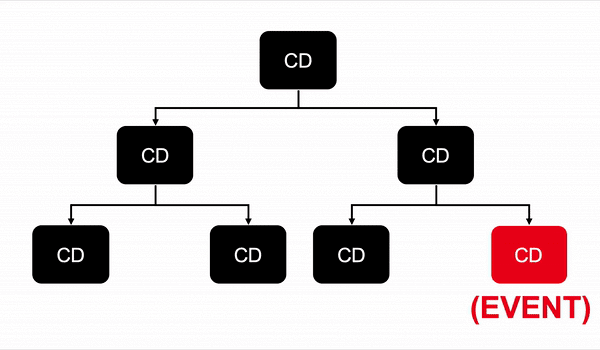
\includegraphics[width=\linewidth]{cycle1.png} \medskip

	\item Change detection checks the component tree top to bottom \medskip
	
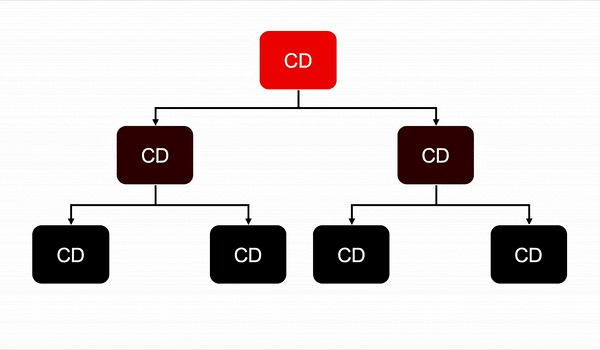
\includegraphics[width=\linewidth]{cycle2.png}
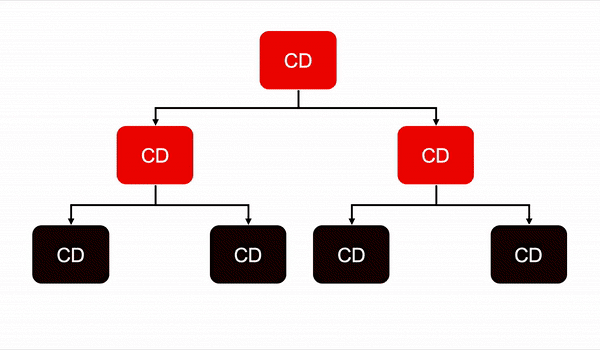
\includegraphics[width=\linewidth]{cycle3.png}
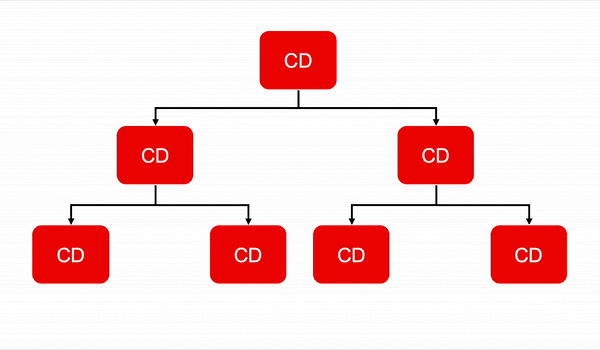
\includegraphics[width=\linewidth]{cycle4.png}
	\autocite{Hoffmann2019}
\end{enumerate}


\subsection{What are the alternatives to the default change detection strategy?}
\label{sec:change_detection_strategies}
There are two major strategies developers can use:
\begin{itemize}
	\item Default
	\item OnPush
\end{itemize}

With the \emph{OnPush} strategy it is possible to skip components when checking the component tree for changes. This can save time when dealing with lots of immutable components.
The images below illustrate the \emph{OnPush} mechanism.
\begin{enumerate}
	\item An event triggers the change detection. \medskip
	
	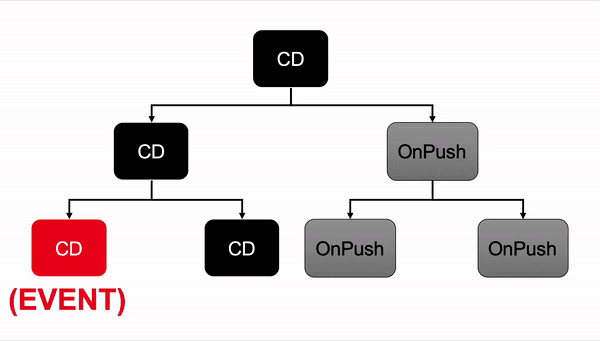
\includegraphics[width=\linewidth]{onpush-cycle1.png} \medskip
	\item Change detection checks the component tree top to bottom, but skips the parts where \emph{OnPush} is used. \medskip
	
	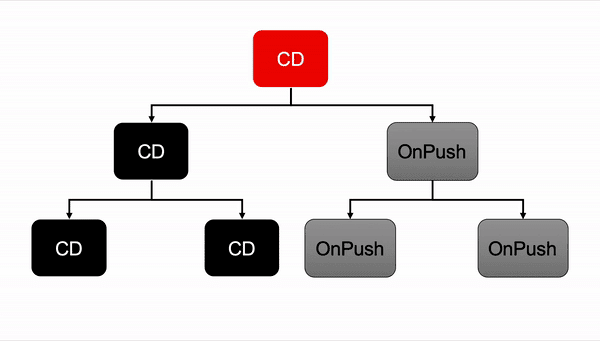
\includegraphics[width=\linewidth]{onpush-cycle2.png}
	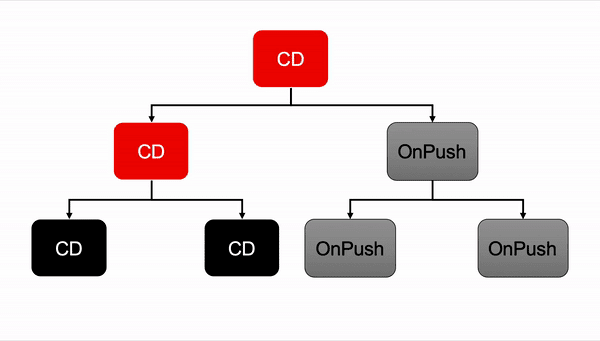
\includegraphics[width=\linewidth]{onpush-cycle3.png}
	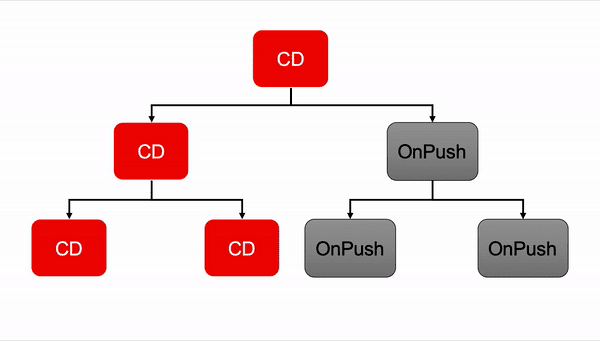
\includegraphics[width=\linewidth]{onpush-cycle4.png}
\autocite{Hoffmann2019}
\end{enumerate}
	
Thanks to the custom strategy implemented by the developer, Angular will not update the components where \emph{OnPush} is defined unless:
\begin{itemize}
	\item The reference of an \emph{@Input} property changes.
	\item An event handler is triggered in the component or one of its children.
	\item An observable that uses the \emph{async} pipe in the template provides a new value.
	\item The change detection is triggered by the developer.
\end{itemize} \medskip
This strategy, where change detection is manually triggered, might be cumbersome and error prone as the developer should import and call the change detection explicitly every time an object's properties might have changed.
Since the release of Angular 9 coming with the brand new Ivy compiler, Zone.js can be excluded from the project and a typescript decorator can handle a manually triggered change detection strategy.
\textcite{Buomprisco2019} uses the \emph{\(\Theta\)cmp} property to get the component definitions processed by Angular at runtime. A component definition is a data structure with many metadata properties used by the Ivy runtime, for example the lifecycle hooks. \autocite{BrinkNielsen2019}  He then used said properties to override the \emph{onInit} and \emph{onDestroy} methods of the decorated component.
In the \emph{onInit} method, his decorator checks for each property if it is an object or an observable. If it is an object, it converts to a proxy and uses Angular Ivy's \emph{\(\Theta\)markdirty} method to mark the component in its handler function. When the property is an observable, it subscribes to the observable and stores the subscription in a list on the component.
% Voor literatuurverwijzingen zijn er twee belangrijke commando's:
% \autocite{KEY} => (Auteur, jaartal) Gebruik dit als de naam van de auteur
%   geen onderdeel is van de zin.
% \textcite{KEY} => Auteur (jaartal)  Gebruik dit als de auteursnaam wel een
%   functie heeft in de zin (bv. ``Uit onderzoek door Doll & Hill (1954) bleek
%   ...'')


%---------- Methodologie ------------------------------------------------------
\section{Methodology}
\label{sec:methodologie}
The first section of the thesis will contain an in-depth analysis of change detection in Angular and a visualization of the change detection process. 
In the second phase, an IoT device (or simulation) will be programmed to send its sensor data to a \emph{signalR hub}. 
Afterwards three basic web applications will be developed to visualize live-data of the IoT device's state in the browser. 
In the first application the default strategy will be used so it relies on Zone.js for triggering change detection. In the second application the \emph{OnPush} strategy will be implemented where Zone.js is manually called to trigger change detection. For the third strategy Zone will be excluded from the project and Ivy's \emph{\(\Theta\)markdirty} method will be used to trigger change detection.
The developer's experience of each strategy can be measured by keeping track of the time it takes to build each application.
At the last phase, the performance of each strategy can be measured and compared when the IoT device fires data to the \emph{signalR hub} with high frequency.  
When the frequency of updates increases, the differences in performance between the scenarios should be distinguishable to the eye. But since numbers tell the tale, performance will be measured using following metrics:
\begin{itemize}
    \item Size of chunks that have to be downloaded
    \item Monetary cost to view the page
    \item Processor usage
    \item Time it takes to see a first paint
    \item Time it takes to see a first meaningful paint
    \item Google's speed index
\end{itemize}
\autocite{Arsenault2017}

%---------- Verwachte resultaten ----------------------------------------------
\section{Expected results}
\label{sec:verwachte_resultaten}
The size of chunks that have to be downloaded should provide a lower number at the third method since there is no need for Zone.js.
This could affect the monetary cost to view the page and processor usage by causing them to give lower thus better results. The time it takes to see a first meaningful paint and the speed index are interesting numbers, since these are the ones that a user notices the most.

%---------- Verwachte conclusies ----------------------------------------------
\section{Expected conclusions}
\label{sec:verwachte_conclusies}
When fewer requests are made, all three scenarios should provide a viable solution with little to no remarkable differences.
As the amount of updates increases and the application is pushed to its limits, the manual strategies (2 and 3) should return better responsiveness as they will not evaluate each component every time an update is fired.
The first scenario should be the easiest to develop as Zone.js worries about change detection.
Once the decorator used in the third scenario is implemented correctly, the manual triggering strategy should also be easy to use for future expansion of the project.



	

%------------------------------------------------------------------------------
% Referentielijst
%------------------------------------------------------------------------------
% TODO: de gerefereerde werken moeten in BibTeX-bestand ``voorstel.bib''
% voorkomen. Gebruik JabRef om je bibliografie bij te houden en vergeet niet
% om compatibiliteit met Biber/BibLaTeX aan te zetten (File > Switch to
% BibLaTeX mode)

\phantomsection
\printbibliography[heading=bibintoc]

\end{document}
